\documentclass[prl,twocolumn]{revtex4-1}

\usepackage{graphicx}
\usepackage{color}
\usepackage{latexsym,amsmath}
\usepackage{amsfonts}
\usepackage{caption}
\usepackage{siunitx}

\definecolor{linkcolor}{rgb}{1.0,0.647,0.0} %hyperlink
\usepackage[pdftex,colorlinks=true, pdfstartview=FitV, linkcolor= linkcolor, citecolor= linkcolor, urlcolor= linkcolor, hyperindex=true,hyperfigures=true]{hyperref} %hyperlink%

\usepackage{enumitem}
\setlist[itemize]{leftmargin=*}


\setcounter{secnumdepth}{2}

\renewcommand{\thesection}{\arabic{section}}
\renewcommand{\theequation}{\thesection.\arabic{equation}}

\makeatletter
\@addtoreset{equation}{section} % Reset equation counter at each section
\makeatother

\begin{document}

\title{Quantum Optics and Laser, Lab4 - Laser dynamics}



\author{Calandra Buonaura Lorenzo}

\date{\today}


\begin{abstract}

This experiment investigates the dynamics of a high-power distributed feedback (DFB) laser module in conjunction with a precision optical power meter to analyze the relationship between electrical input and optical output. Using the G\&H AA1401 DFB laser module and the Thorlabs PM16-122 power meter, we explore the behavior of the laser's light-current (LI) and voltage-current (VI) characteristics, as well as the efficiencies that define its performance. The experimental setup combines stability, precision, and adaptability, allowing for detailed insights into efficiency parameters such as differential efficiency, wall-plug efficiency, and slope efficiency.

\end{abstract}

\maketitle

\section{Introduction}

The study of laser dynamics is fundamental in understanding and optimizing the performance of laser systems for applications ranging from telecommunications to precision sensing. At the core of this analysis lies the characterization of key operational parameters, including the relationship between electrical input (current and voltage) and optical output (power), as well as efficiency metrics that gauge the system's overall performance. This characterization not only highlights the laser's operational thresholds but also identifies factors that influence its efficiency, such as thermal effects and saturation. In this work, we utilize a G\&H AA1401 series high-power DFB laser module, which offers high stability, narrow linewidth, and polarization-maintaining capabilities, making it suitable for a wide range of optical experiments. The laser is paired with a Thorlabs PM16-122 power meter, a versatile device capable of precise low-power measurements across a broad wavelength range. Together, these components form an experimental setup that is both robust and adaptable, facilitating detailed exploration of laser behavior under varying conditions. The analysis focuses on the light-current (LI) and voltage-current (VI) characteristics of the laser diode, which reveal essential details about its performance in both the spontaneous emission and stimulated emission regimes. Efficiency metrics are calculated to evaluate the effectiveness of electrical-to-optical power conversion.

\section{Theoretical Framework}

When studying laser dynamics, it's important to describe the relationship between the electrical input (current and voltage) and the optical output (power), focusing on the efficiency and the behaviours within the operational range of the laser.

\subsection{LI curve}

In laser diodes, the light output power (\(P_{\text{opt}}\)) typically increases with the injected current (\(I\)) above a certain threshold current (\(I_{\text{th}}\)), marking the onset of lasing~\cite{pap1}. Below \(I_{\text{th}}\), the laser operates in the spontaneous emission regime, where the output power remains negligible.

Above \(I_{\text{th}}\), the output power increases linearly with the current, and the slope of this linear region is referred to as the \textit{slope efficiency}, which indicates how effectively the injected current is converted into optical power. The general behavior of the LI curve can be summarized as:

\begin{equation}
\label{eq:fit_LI_curve}
P_{\text{opt}}(I) = \eta_d \cdot (I - I_{\text{th}}),
\end{equation}

where \(\eta_d\) is the differential efficiency.

\subsection{VI curve}

The voltage across the laser diode (\(V\)) typically increases with the injected current, but the relationship is non-linear~\cite{pap1}. This is because at higher currents, thermal effects become significant, leading to a reduction in slope and potential saturation. The voltage-current characteristic can be modeled as:

\begin{equation}
\label{eq:fit_VI_curve}
V(I) = V_{\text{th}} + R_{\text{diode}} \cdot I,
\end{equation}

where \(V_{\text{th}}\) is the threshold voltage, and \(R_{\text{diode}}\) is the dynamic resistance of the diode.

\subsection{Power-Voltage relationship}

The power (\(P_{\text{opt}}\)) and voltage (\(V\)) are related through the injected current (\(I\)): as the current increases, both the output power and voltage increase. However, thermal effects and saturation may reduce the efficiency of the laser at higher currents, leading to a deviation in the expected power-voltage relationship.

The total electrical power \(P_{\text{elec}}\) delivered to the laser is given by:

\begin{equation}
P_{\text{elec}} = V \cdot I,
\end{equation}

and the optical output power is related to the electrical power as:

\begin{equation}
P_{\text{opt}} = \eta_w \cdot P_{\text{elec}},
\end{equation}

where \(\eta_w\) is the \textit{wall-plug efficiency}, which describes the overall conversion of electrical power into optical power, accounting for all losses in the system~\cite{pap2}.

At higher injection currents, the optical output power $P_{\text{opt}}$ tends to saturate due to thermal effects, carrier recombination, and gain saturation within the laser medium. These phenomena can be described by the exponential saturation model, which modifies the linear relationship between current and output power. The model is given by:

\begin{equation}
\label{eq:fit_wpe}
P_{\text{opt}}(I) = \frac{A}{1 + B \exp(-C I)},
\end{equation}

where $A$, $B$, and $C$ are constants that characterize the laser's behavior.

This model introduces a correction factor, $\left( 1 + B \exp(-C I) \right)^{-1}$, which accounts for the decreasing efficiency as the current approaches saturation. At low currents, the exponential term becomes negligible, and the output power follows the linear relationship. However, as the current increases, the exponential term suppresses the output, modeling the saturation behavior observed in practice.

\subsection{Efficiency calculations}

As already pointed out, there are different efficiencies that can be calculated when analyzing the total power of a laser; for a clearer presentation of the topic, they are reported in the following:

\begin{itemize}
    \item \textbf{Differential efficiency (\(\eta_d\)):}
        Differential efficiency measures the incremental change in optical output power (\(P_{\text{opt}}\)) for an incremental change in drive current (\(I\)) above the threshold current (\(I_{\text{th}}\)):

        \begin{equation}
        \eta_d = \frac{\Delta P_{\text{opt}}}{\Delta I}.
        \end{equation}

        This is the slope of the linear region of the LI curve and is typically expressed in units of mW/mA. It represents the effectiveness of the laser in converting electrical current into optical power after reaching the threshold current.

    \item \textbf{Wall-Plug efficiency (\(\eta_w\)):}
        Wall-plug efficiency describes the overall conversion efficiency of electrical input power (\(P_{\text{elec}}\)) into optical output power (\(P_{\text{opt}}\)):

        \begin{equation}
        \eta_w = \frac{P_{\text{opt}}}{P_{\text{elec}}} = \frac{P_{\text{opt}}}{V       \cdot I}.
        \end{equation}

        This efficiency accounts for all losses in the laser system, including thermal losses and internal inefficiencies, and is a critical parameter for evaluating the performance of a laser device.

    \item \textbf{Slope Efficiency}

        Slope efficiency is a subset of differential efficiency and is specifically calculated for the linear lasing region. It represents the laser's ability to convert electrical power into optical power within the operational range of the laser, especially after reaching threshold:

        \begin{equation}
        \eta_{\text{slope}} = \frac{dP_{\text{opt}}}{dI}.
        \end{equation}
        
        Slope efficiency is typically high in the linear region and can provide insight into how well the laser is performing in terms of converting electrical energy into optical output.
\end{itemize}


\section{Apparatus}

The experimental setup consists of a high-power distributed feedback (DFB) laser module and a PM16-122 power meter for optical power measurement, which is then interfaced with a computer for data acquisition. Below, the components are described in detail:

\begin{enumerate}
    \item \textbf{High-power DFB laser module (G\&H AA1401 Series):}
    The G\&H AA1401 series high-power DFB laser is an InGaAs/InP multi-quantum well (MQW) laser diode designed for applications requiring low relative intensity noise (RIN), stable polarization-maintaining properties, and high reliability~\cite{pap4}. It features:
    \begin{itemize}[noitemsep]
        \item \textbf{Wavelength range:} Covers \SI{1537}{\nano\meter} to \SI{1565}{\nano\meter} (C-band) and \SI{1565}{\nano\meter} to \SI{1617}{\nano\meter} (L-band), supporting ITU grid wavelengths with 50 or 100 GHz spacing.
        \item \textbf{Output power:} From \SI{40}{\milli\watt} to \SI{100}{\milli\watt}, allowing the system to be tuned for both high-sensitivity and high-power applications.
        \item \textbf{Linewidth:} \SI{1}{\mega\hertz}, suitable for applications requiring narrow spectral lines, such as precision metrology or coherent detection.
        \item \textbf{Polarization extinction ratio (PER):} Ranges from \SI{17}{\decibel} to \SI{21}{\decibel}, providing excellent polarization stability, which is critical in experiments involving birefringent components or polarization-sensitive measurements.
        \item \textbf{Integrated components:} A thermoelectric cooler (TEC) for precise temperature control, a thermistor for feedback, and a monitor photodiode for real-time power measurements. These integrations simplify operation and reduce the need for external instrumentation.
        \item \textbf{Fiber and connector:} Polarization-maintaining (PM) or single-mode (SM) fiber with FC/APC connectors, ensuring compatibility with optical systems and reliability during long-term usage.
        \item \textbf{Advanced features:} Laser-welded, hermetically sealed design for durability; optional Bias-T for RF applications; and tested to Telcordia GR-468 Core/MIL-STD-883 standards for reliability. These features make the module a dependable choice for both experimental and industrial environments.
    \end{itemize}
    The laser is operated at a chip temperature of \SI{25}{\degreeCelsius} with a typical drive current of \SI{350}{\milli\ampere}. Its compact design and built-in temperature control mechanisms minimize environmental sensitivity, enhancing reproducibility and experimental confidence.

    \item \textbf{Optical Power Meter (Thorlabs PM16-122):}
    The PM16-122 power meter is equipped with a Germanium photodiode sensor optimized for precise low-power optical measurements, which makes it an ideal counterpart to the high-power DFB laser~\cite{pap5}. Key specifications include:
    \begin{itemize}[noitemsep]
        \item \textbf{Wavelength range:} \SI{700}{\nano\meter} to \SI{1800}{\nano\meter}, ensuring compatibility with the laser's output and offering versatility for future experimental configurations.
        \item \textbf{Power range:} \SI{50}{\nano\watt} to \SI{40}{\milli\watt}, accommodating both faint signals and moderate-power beams, which is particularly useful in dynamic experiments with varying conditions.
        \item \textbf{Active detector area:} \SI{9.7}{\milli\meter} $\times$ \SI{9.7}{\milli\meter} with a \SI{9.5}{\milli\meter} input aperture. This large detector area simplifies alignment and reduces the risk of measurement errors due to beam clipping.
        \item \textbf{Calibration accuracy:} NIST- and PTB-traceable spectral calibration data stored in non-volatile memory, with an uncertainty of \(\pm 5\%\). This ensures reliable data over extended periods.
        \item \textbf{Dynamic range:} Automatic range selection for optimal accuracy; resolution better than \SI{2}{\nano\watt}. This capability makes it possible to measure subtle power fluctuations with high precision.
        \item \textbf{Response time:} Less than \SI{1}{\micro\second}, allowing real-time measurements and enabling fast feedback loops in dynamic systems.
        \item \textbf{Mounting compatibility:} SM1-threaded housing for lens tubes, apertures, and optical adapters, along with 8-32 and M4 threaded mounting holes. This design facilitates easy integration into complex setups.
    \end{itemize}
\end{enumerate}

The combination of the G\&H AA1401 series DFB laser and the Thorlabs PM16-122 power meter reflects a deliberate choice of components that complement each other. The laser provides stable, high-quality output, while the power meter ensures precise measurements across a broad dynamic range. This synergy allows the setup to meet the dual demands of flexibility and accuracy, which are critical in advanced optical experiments. The DFB laser output is coupled into the PM16-122 power meter using a PM fiber with an FC/APC connector and the laser module's TEC stabilizes the operating temperature at \SI{25}{\degreeCelsius}, optimizing spectral performance and output power. A removable VIS/IR viewing target aids in beam alignment, ensuring optimal focus onto the detector. The entire setup is monitored and controlled through software interfacing with the computer (see Figure~\ref{fig:setup}).

\begin{figure}
    \centering
    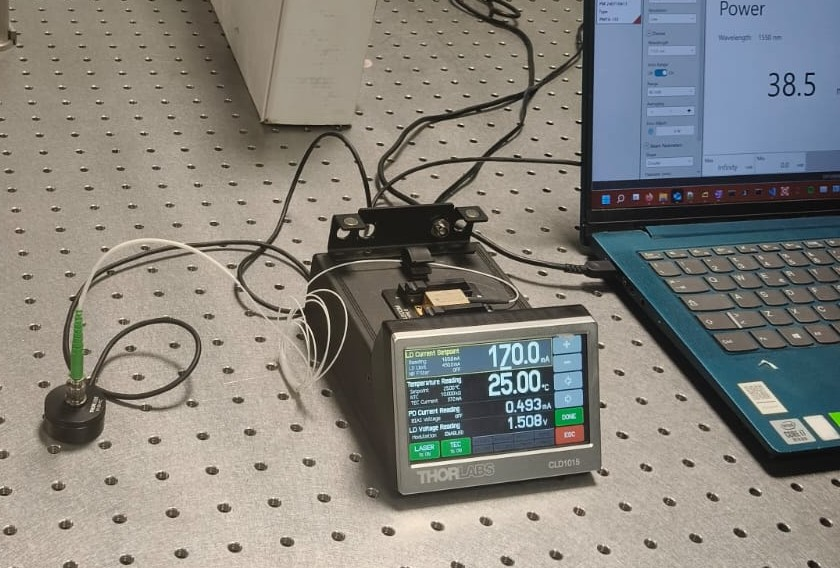
\includegraphics[width=\linewidth]{Images/setup.jpg}
    \caption{Experimental setup, featuring the DFB laser module and the PM16-122 power meter.}
    \label{fig:setup}
\end{figure}


\section{Results}
As previously anticipated, the analysis in the experiment focuses on the relationship between current, voltage and power.

\subsection{LI curve and slope efficiency}
First of all, we can leverage the current and the output power to study the LI curve, which is presented in Figure~\ref{fig:LI_curve}. We can clearly see that there are two regimes: the first up to a certain threshold current, with $P\approx0$, and the second after the threshold current with a linear behaviour. First of all we need to find the threshold current and verify that it's coherent with the expectation ($I_{th} \approx \SI{400}{\milli\ampere}$); in order to do so, we can do two linear fit for the two regimes and find where the two lines meet. From this analysis we get that $I_{th} = (441 \pm 9) \SI{}{mA}$, which has the same order of magnitude of the expected result; from the datasheet we can see that we are inside the expected window (which is $350-500\SI{}{\milli\ampere}$). This result will be used for the following analysis: with more data in the critical region we could find a more accurate result, but in any case this is enough for the purpose of this analysis.

\begin{figure}[!t]
    \centering
    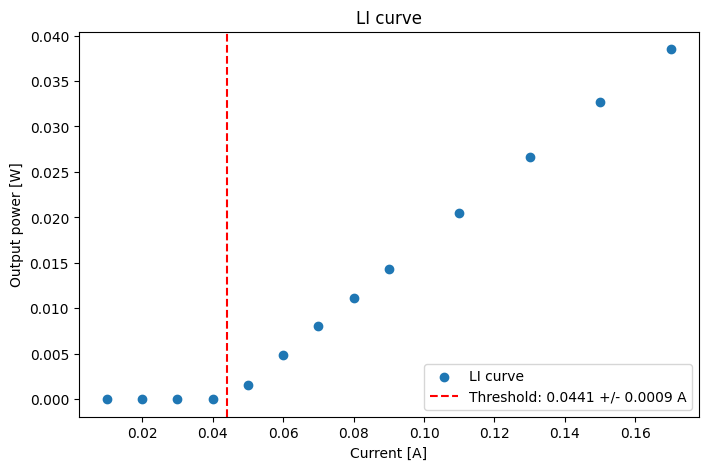
\includegraphics[width=\linewidth]{Images/LI_curve.png}
    \caption{LI curve.}
    \label{fig:LI_curve}
\end{figure}

After this initial analysis, we can perform a linear fit (see Equation~\eqref{eq:fit_LI_curve}) on the lasing region and find the differential efficiency of this setup: Figure~\ref{fig:LI_curve_fit} shows the result of this procedure. First of all we can see that we have a very good fit (as expected): then, from the fit we obtain that we have a differential efficiency of $308.19 \pm 1.75 \SI{}{\milli\watt}/\SI{}{\milli\ampere}$. This result is compatible with the expected differential efficiency for a DFB laser module, so we can conclude that the setup used works fine and we can proceed with the analysis. 

\begin{figure}[!b]
    \centering
    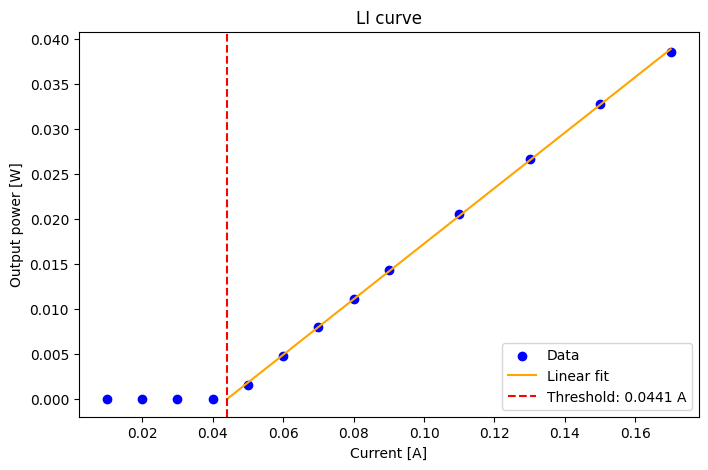
\includegraphics[width=\linewidth]{Images/LI_curve_fit.png}
    \caption{Fitting of the lasing region of the LI curve using a linear relation.}
    \label{fig:LI_curve_fit}
\end{figure}

\subsection{VI curve}
Then, we can proceed analyzing the VI curve: we expect a non-linear relation, which is what we get and it's depicted in Figure~\ref{fig:VI_curve_fit}. We can see that in correspondence of the threshold current we get a change in the slope of the line, which gets less steep as the current increases. This is again in agreement with what expected (see Equation~\eqref{eq:fit_VI_curve}), as for higher currents we have that thermal effects become more significant. We don't see any saturation in this case because we don't reach a very high current; otherwise, we would expect another change in slope up to a constant value, due to the saturation effect.

\begin{figure}[!t]
    \centering
    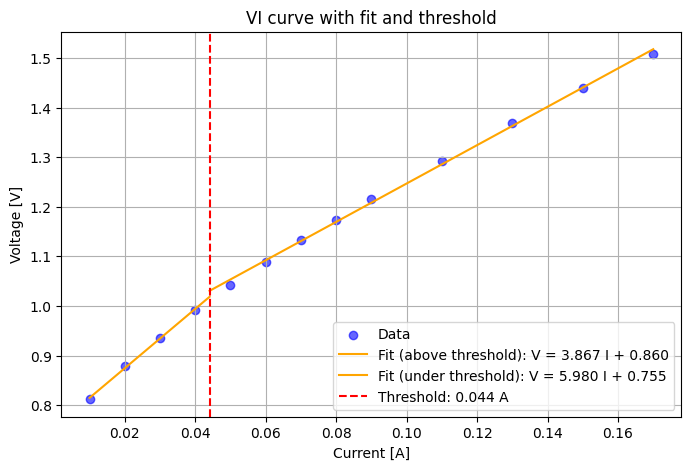
\includegraphics[width=\linewidth]{Images/VI_curve_fit.png}
    \caption{Fitting of the non-lasing and lasing region of the VI curve using a linear relation.}
    \label{fig:VI_curve_fit}
\end{figure}


\subsection{Wall-Plug efficiency}

\begin{figure}[!b]
    \centering
    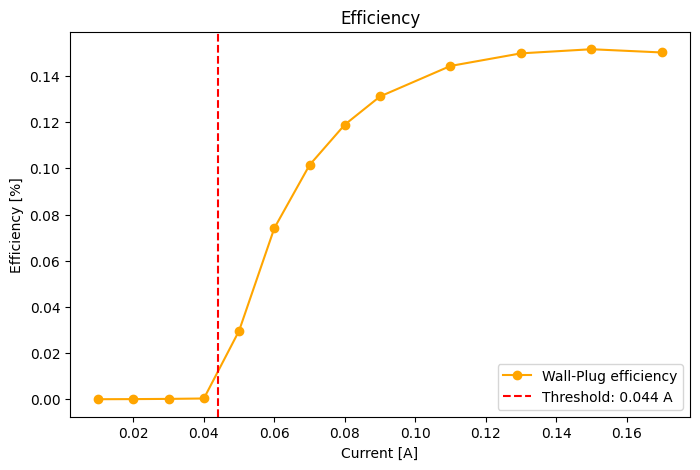
\includegraphics[width=\linewidth]{Images/wpe.png}
    \caption{Wall-Plug efficiency.}
    \label{fig:wpe}
\end{figure}

Finally, the Wall-Plug efficiency has been studied: also in this case we can see that we have a change in the behaviour when we reach the threshold current, passing from zero to a linear dependency. However, in this case, we see that we have a saturation effect after a certain value of the current, as the efficiency doesn't increase anymore: this means that the overall conversion of electrical power into optical
power becomes a constant value (due to the loss of the system). This is in agreement with the exponential saturation model, so we can perform a fit using Equation~\eqref{eq:fit_wpe} to find the best parameters. Figure~\ref{fig:wpe_fit} shows the fit, which seems coherent in the lasing regime; the best parameter found are $A = (0.147 \pm 0.003) \%$, $B = 672.95 \pm 476.79$, $C = 104.17 \pm 11.56 \SI{}{\ampere}^{-1}$. 

The physical interpretation of these values is the following:

\begin{itemize}
    \item A: this constant represents the maximum optical output power that the laser can achieve, as it's clear from Figure~\ref{eq:fit_wpe}.
    \item B: this constant determines the rate of the saturation effect, so it governs how quickly the output power approaches saturation as the injection current increases.
    \item C: this constant controls the current dependence of the saturation effect, thus it dictates how rapidly the exponential term decays as current increases
\end{itemize}

Overall the behaviour is in agreement with what expected, with the WPE that shows the saturation effect for high value of the current.

\begin{figure}[!t]
    \centering
    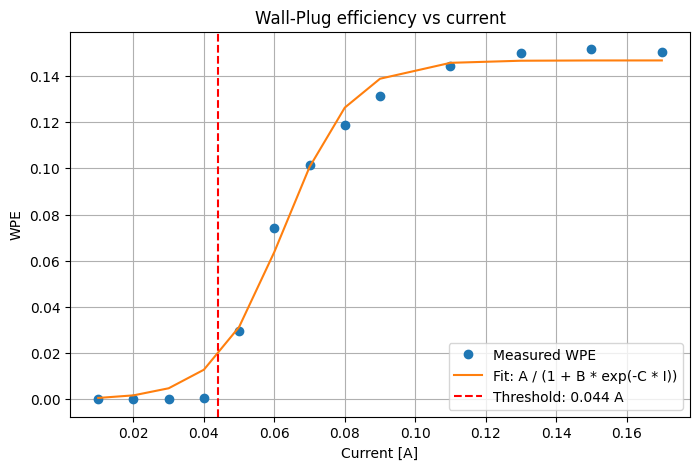
\includegraphics[width=\linewidth]{Images/wpe_fit.png}
    \caption{Fit of the WPE using the exponential saturation model.}
    \label{fig:wpe_fit}
\end{figure}



\section{Conclusions}

In this work, we have presented a detailed analysis of the laser characteristics, focusing on the relationship between current, voltage, and optical power.

First, we analyzed the LI curve and identified two distinct regimes: a sub-threshold regime where the optical output power is negligible and a lasing regime where the power increases linearly with current. The threshold current was found to be \(I_{\text{th}} = (441 \pm 9) \, \text{mA}\), which is consistent with the expected value from the datasheet. The differential efficiency, calculated from the lasing region of the LI curve, was determined to be \(308.19 \pm 1.75 \, \text{mW/mA}\), which is in agreement with the typical differential efficiency for a DFB laser module.

The analysis of the VI curve revealed the expected non-linear behavior with a change in slope at the threshold current, consistent with thermal effects becoming more significant at higher currents. Although saturation effects were not observed, the general trend aligns with expectations.

Finally, the Wall-Plug efficiency (WPE) curve showed a similar trend with a change in behavior at the threshold current, followed by a saturation effect at higher currents. The exponential saturation model provided a good fit to the data, with parameters that are consistent with the expected physical behavior of the laser. The constants obtained from the fit, \(A\), \(B\), and \(C\), were interpreted in terms of the maximum optical output power, the rate of the saturation effect, and the current dependence of the saturation effect, respectively.

Overall, the experimental setup and analysis were successful in capturing the key characteristics of the laser's performance, confirming that the setup works as expected.

\section{Code}
All the data and the code for the data analysis can be found in this public Github repository: \href{https://github.com/Kallo27/QOL/tree/main/Lab4}{https://github.com/Kallo27/QOL/tree/main/Lab4}

\begin{thebibliography}{99}

\bibitem{pap1}
S. E. Miller, \textit{Laser efficiency and threshold phenomena}, Journal of Applied Physics, (1962).

\bibitem{pap2}
P. W. Epworth, \textit{Wall-Plug efficiency of laser systems: analysis and optimization}, IEEE Journal of Quantum Electronics (1984).

\bibitem{pap3}
E. J. Murphy and P. R. Grant, \textit{Modeling saturation in semiconductor lasers}, Optics Express (2006).

\bibitem{pap4}
Gooch \& Housego, \textit{High Power DFB Laser – AA1401 Series}, Datasheet Rev. 13.2, March 2022. Available: \url{https://www.goochandhousego.com}.

\bibitem{pap5}
Thorlabs, Inc., \textit{PM16-122 Power Meter Specifications}, Datasheet Rev. A, May 2015. Available: \url{https://www.thorlabs.com}.

\end{thebibliography}


\end{document}
